% You should title the file with a .tex extension (hw1.tex, for example)
\documentclass[a4paper, 11pt]{article}

\usepackage{amsmath}
\usepackage{amssymb}
\usepackage{fancyhdr}
\usepackage{graphicx}

\usepackage[margin=1in]{geometry}

\newcommand{\question}[2] {\vspace{.25in} \hrule\vspace{0.5em}
	\noindent{\bf #1: #2} \vspace{0.5em}
	\hrule \vspace{.10in}}
\renewcommand{\part}[1] {\vspace{.10in} {\bf (#1)}}

\newcommand{\myname}{Possawat Sanorkam}
\newcommand{\myemail}{possawat2017@hotmail.com}
\newcommand{\myhwnum}{1}

\setlength{\parindent}{0pt}
\setlength{\parskip}{5pt plus 1pt}

\pagestyle{fancyplain}
\lhead{\fancyplain{}{\textbf{HW\myhwnum}}}      % Note the different brackets!
\rhead{\fancyplain{}{\myname\\ \myemail}}
\chead{\fancyplain{}{ICCS310}}

\begin{document}
	
	\medskip                        % Skip a "medium" amount of space
	% (latex determines what medium is)
	% Also try: \bigskip, \littleskip
	
	\thispagestyle{plain}
	\begin{center}                  % Center the following lines
		{\Large ICCS310: Assignment \myhwnum} \\
		\myname \\
		\myemail \\
		\today \\
	\end{center}
	
	\question{1}{Review: Something About Sets} %don't delete yet:(}
	
	\part{1} Let $A_1, A_2, A_3$ be any sets from a universe $\mathcal{U}$. 
	 {\em Prove that $ \overline{A_1 \cup A_2 \cup A_3} = \overline{A_1} \cap \overline{A_2} \cap \overline{A_3}$.}\\
	
	{\em Proof}: We want to show that $\overline{A_1 \cup A_2 \cup A_3} \subseteq \overline{A_1} \cap \overline{A_2} \cap \overline{A_3}$
	and $\overline{A_1} \cap \overline{A_2} \cap \overline{A_3} \subseteq \overline{A_1 \cup A_2 \cup A_3} $
	
	Let $A_1, A_2, A_3$ be any three given sets. We'll first prove that
	$\overline{A_1 \cup A_2 \cup A_3} \subseteq \overline{A_1} \cap \overline{A_2} \cap \overline{A_3}$.
	Let $x \in \overline{A_1 \cup A_2 \cup A_3}$. Then, $x \notin A_1 \cup A_2 \cup A_3$ by the definition of complement, so then $x \notin A_1$, $x \notin A_2$ and $x \notin A_3$, by the definition of union. This means that $x \in \overline{A_1}$, $x \in \overline{A_2}$, and $x \in \overline{A_3}$, by the definition of complement. 
	Hence, $x \in \overline{A_1} \cap \overline{A_2} \cap \overline{A_3}$ 
	since x is in $\overline{A_1} $, $ \overline{A_2} $, and $ \overline{A_3}$.

	Also, we will show that $\overline{A_1} \cap \overline{A_2} \cap \overline{A_3} \subseteq \overline{A_1 \cup A_2 \cup A_3} $. Let $y \in \overline{A_1} \cap \overline{A_2} \cap \overline{A_3}$, so y is in $\overline{A_1} $, $ \overline{A_2} $, and $ \overline{A_3}$, by the definition of intersection. 
	This means $y \notin A_1$, $y \notin A_2$, and $y \notin A_3$, by the definition of complement. It follows that $y \notin A_1 \cup A_2 \cup A_3$, and so $y \in \overline{A_1 \cup A_2 \cup A_3}$.
	
	In conclusion, $ \overline{A_1 \cup A_2 \cup A_3} = \overline{A_1} \cap \overline{A_2} \cap \overline{A_3}$. $\square$
	
	
	\part{2} Let A and B be any sets from a universe $\mathcal{U}$. 
	{\em Prove that $ \overline{A \cup B} = \overline{A} \cap \overline{B}$.}\\
	
	{\em Proof}: We want to show that $\overline{A \cup B} \subseteq \overline{A} \cap \overline{B}$
	and $\overline{A} \cap \overline{B} \subseteq \overline{A \cup B} $
	
	Let $A \text{ and } B$ be any two given sets. We'll first prove that
	$\overline{A \cup B} \subseteq \overline{A} \cap \overline{B}$.
	Let $x \in \overline{A \cup B}$. Then, $x \notin A \cup B$ by the definition of complement, so then $x \notin A$, and $x \notin B$, by the definition of union. This means that $x \in \overline{A}$, and $x \in \overline{B}$, by the definition of complement. 
	Hence, $x \in \overline{A} \cap \overline{B}$ 
	since x is in $\overline{A} $ and $ \overline{B}$.
	
	Also, we will show that $\overline{A} \cap \overline{B} \subseteq \overline{A \cup B} $. Let $y \in \overline{A} \cap \overline{B}$, so y is in $\overline{A} $ and $ \overline{B}$, by the definition of intersection. 
	This means $y \notin A$ and $y \notin B$, by the definition of complement. It follows that $y \notin A \cup B$, and so $y \in \overline{A \cup B}$.
	
	In conclusion, $ \overline{A \cup B} = \overline{A} \cap \overline{B}$. $\square$

	
	\question{2}{Prime and Irrational}
	
	\part{1} Let $p \geq 2$ be a prime and a be a positive integer. Prove that if $p  \text{ divides } a^2$, then $p \text{ divides } a$.\\
	
	{\em Proof}: Using contraposition, we can prove that if $p \text{ does not divides } a$, then $p \text{ does not divides } a^2$ instead.
	
	Let $a$ be any number that cannot be divided by p, so $ a = (p*q) + r$ where $r < p$ and $r,q \in \mathbb{I^+}$. So, we have $a^2 = ((p*q) + r)^2 = (p*q)^2 + 2*(p*q*r) + r^2$. We can see that $r^2$ cannot be divided by $p$. Hence, $p \text{ does not divides } a^2$. 
	
	Therefore, if $p  \text{ divides } a^2$, then $p \text{ divides } a$. $\square$ \\
	
	\part{2} Prove that if $p$ is any positive prime number, then $\sqrt{p}$ is irrational.\\
	
	{\em Proof}: Assume for the sake of contradiction, let $\sqrt{p}$ be a rational number and p is any positive prime number. Then, $\sqrt{p}=a/b$ where $a$ and $b$ are integers and $b \neq 0$.
	\begin{eqnarray}
	\sqrt{p}&=&a/b\\
	p&=&a^2/b^2\\
	p*b^2&=&a^2
	\end{eqnarray}
	From observation, $p$ divides $a^2$ and that means $p$ divide $a$ (Lemma 2.1).
	Let $a = bq$ for some $q \in \mathbb{I^+}$ and plug it back into equation 3.
	\begin{eqnarray}
	p*b^2&=&p^2q^2\\
	b^2&=&pq^2
	\end{eqnarray}
	From observation, $p$ divides $b^2$ and that means $p$ divide $b$ (Lemma 2.1).
	Since we showed that $	p=a^2/b^2 $ but p is a common factor of $a$ and $b$. We can
	conclude that the equation is false and our assumption is contradicting.
	Hence, $\sqrt{p}$ is irrational.
	Therefore, if $p$ is any positive prime number, then $\sqrt{p}$ is irrational. $\square$
	
	\question{3}{Spacing}
	
	Prove that in any set of $n +1$ numbers from $\{1, . . . , 2n\}$, there are always two numbers that are consecutive.
	
	{\em Proof}: Assume for the sake of contradiction that there is no two numbers that are consecutive given any set of $n +1$ numbers from $\{1, . . . , 2n\}$. Let $A$ be the set of $n +1$ numbers from $\{1, . . . , 2n\}$. Using pigeonhole principle, the required size of $A$ is too large to prevent consecutive numbers because the when the size of $A$ is n we could use the set of odd natural number or even natural number where all elements in $A$ is less than $n$. However, the last number to be added will contradict to our assumption that no two numbers are consecutive since there would be no other number to pick, except the consecutive number from $\{1, . . . , 2n\}$. Hence, $A$ is contradicting to our assumption.
	
	Therefore, any set of $n +1$ numbers from $\{1, . . . , 2n\}$, there are always two numbers that are consecutive.$\square$
	
	
	\question{4}{Curious Fact about Graphs}
	
	Let $G = (V, E )$ be an undirected graph. Show that G contains two nodes that have equal degrees.
	
	{\em Proof}: Without loss of generality, assume for the sake of contradiction that $G$ is an undirected graph with no loops which has $n$ vertices and every vertices have different degrees. Let D be the set of degrees for each vertex, $D = \{d_1, d_2, d_3, \dots , d_n\}$. Then, $D = \{0,2,...,n-1\}$, since the number of degree is between $0$ to $n-1$.  From observation, we have that there is a vertex with degree $n-1$ and a vertex with degree $0$ which is not possible for any undirected graph. Hence, $D$ contradicted to what we assumed.
	
	Therefore, if $G = (V, E )$ is an undirected graph, then $G$ contains two nodes that have equal degrees.$\square$
	
	\question{5}{Basic DFAs}
	Let $\sum = \{a, b, c\}$.
	
	\part{1} The language of strings on $\sum$ whose length is divisible by 5.
	
	{\em Solution}:
	\begin{figure}[htbp]
		\centering
		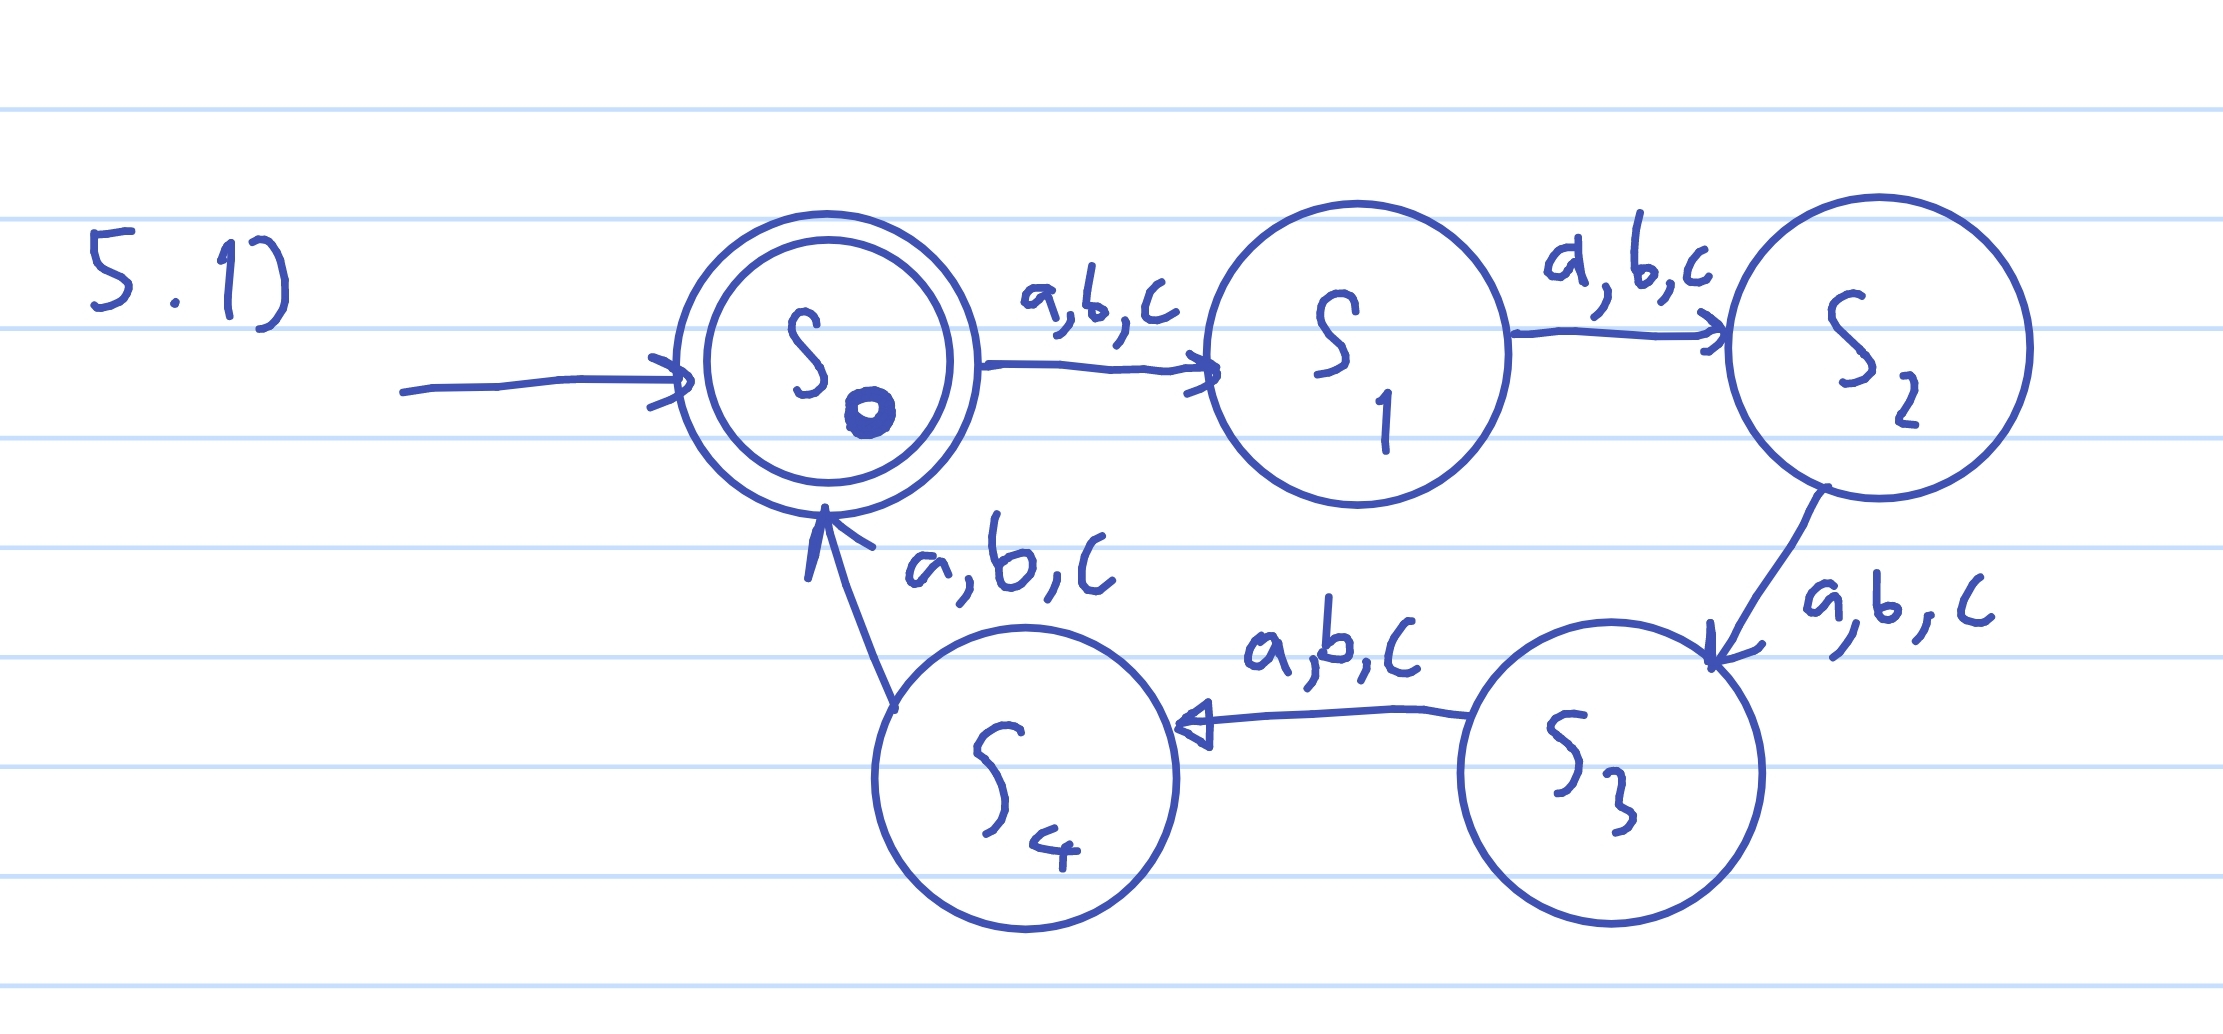
\includegraphics[width=\linewidth]{figures/1.jpg}
	\end{figure}
	
	Let n be the length of the input string.
	
	$S_0$ represents the state where $0 \pmod{5} \equiv n$.\\
	$S_1$ represents the state where $1 \pmod{5} \equiv n$.\\
	$S_2$ represents the state where $2 \pmod{5} \equiv n$.\\
	$S_3$ represents the state where $3 \pmod{5} \equiv n$.\\
	$S_4$ represents the state where $4 \pmod{5} \equiv n$.
	
	So, the accepting state is $S_0$ since this state means the length is divisible by 5.
		
	\part{2} The language of strings on $\sum$ whose length is either even or divisible by 5 (or both).
	
	{\em Solution}:
	
	\begin{figure}[htbp]
		\centering
		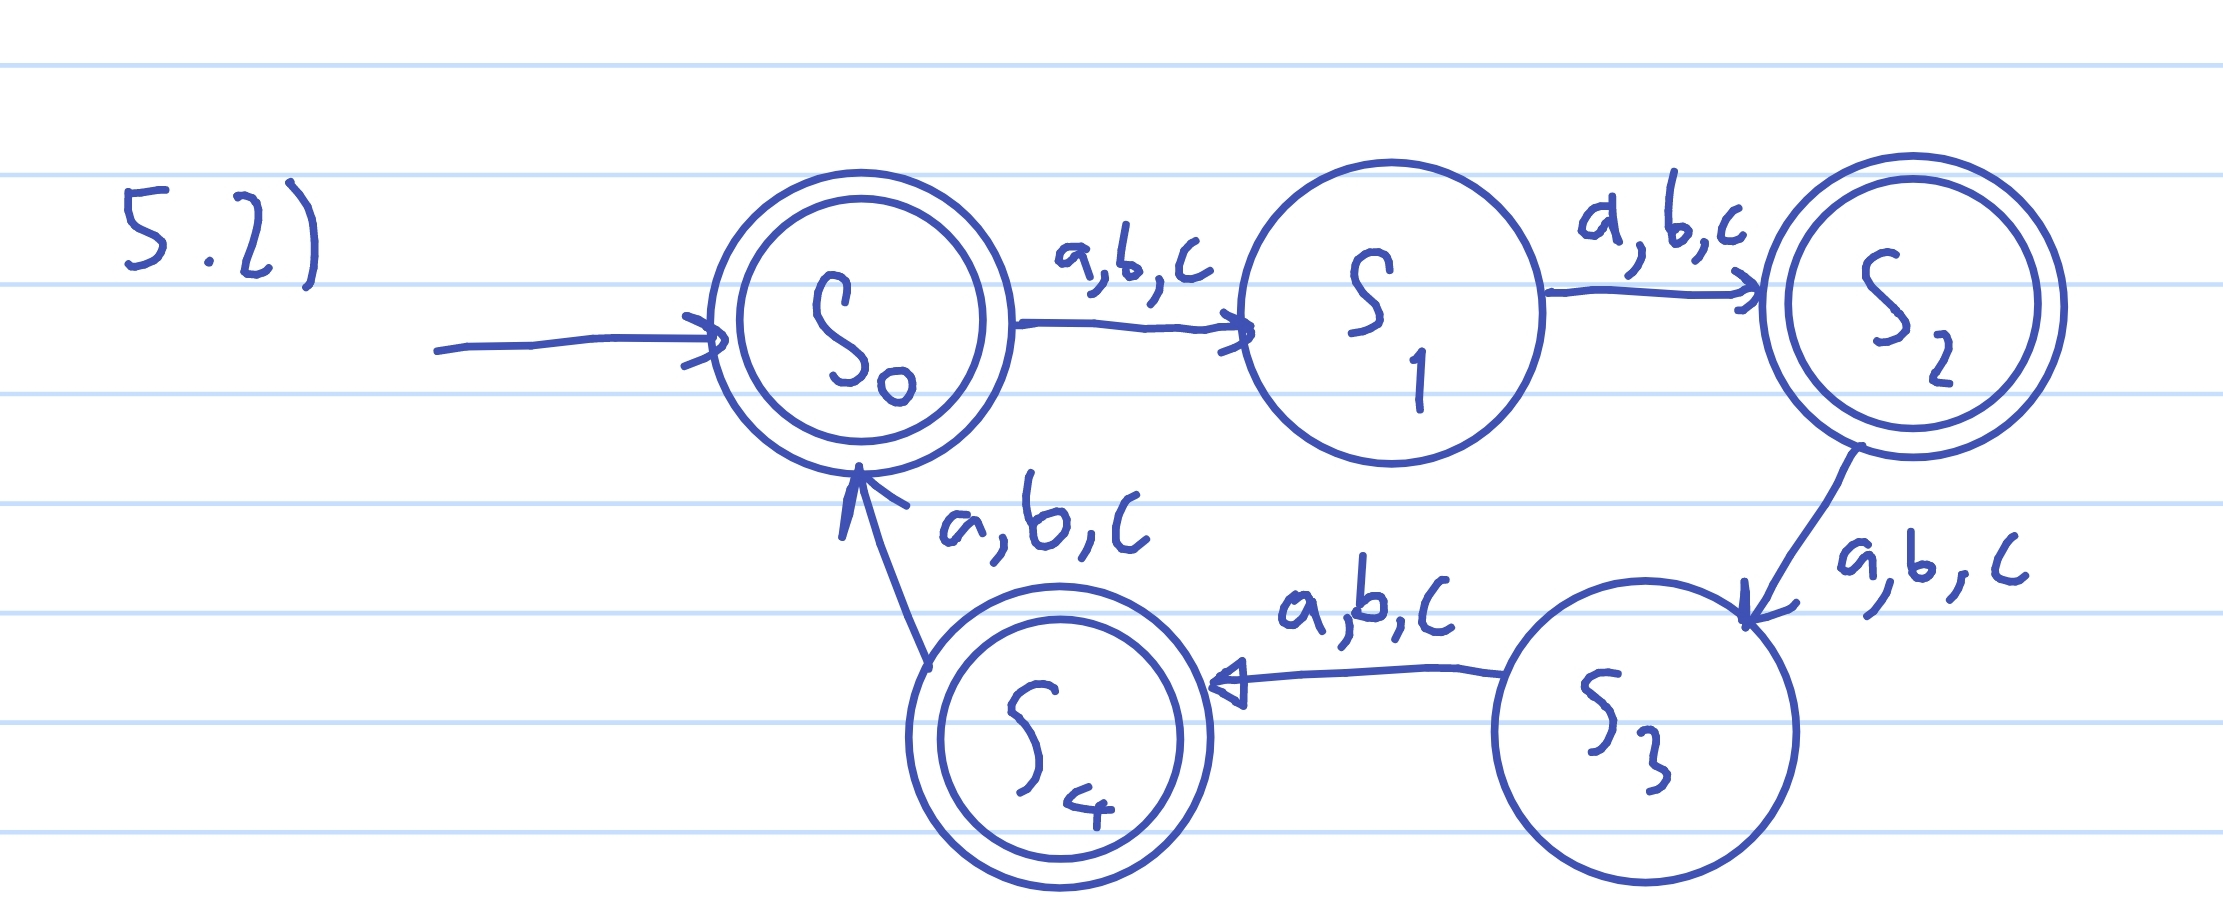
\includegraphics[width=\linewidth]{figures/2.jpg}
	\end{figure}
	Let $n$ be the length of the input string.
	
	$S_0$ represents the state where $0 \pmod{5} \equiv n$.\\
	$S_1$ represents the state where $1 \pmod{5} \equiv n$.\\
	$S_2$ represents the state where $2 \pmod{5} \equiv n$.\\
	$S_3$ represents the state where $3 \pmod{5} \equiv n$.\\
	$S_4$ represents the state where $4 \pmod{5} \equiv n$.
	
	So, the accepting state is $S_0, S_2, S_4$ since this state means the length is either even or divisible by 5
	
	\part{3} The language of strings on $\sum$ that has at least one a and contains an even number of $b$s.
	
	{\em Solution}:
	\begin{figure}[htbp]
		\centering
		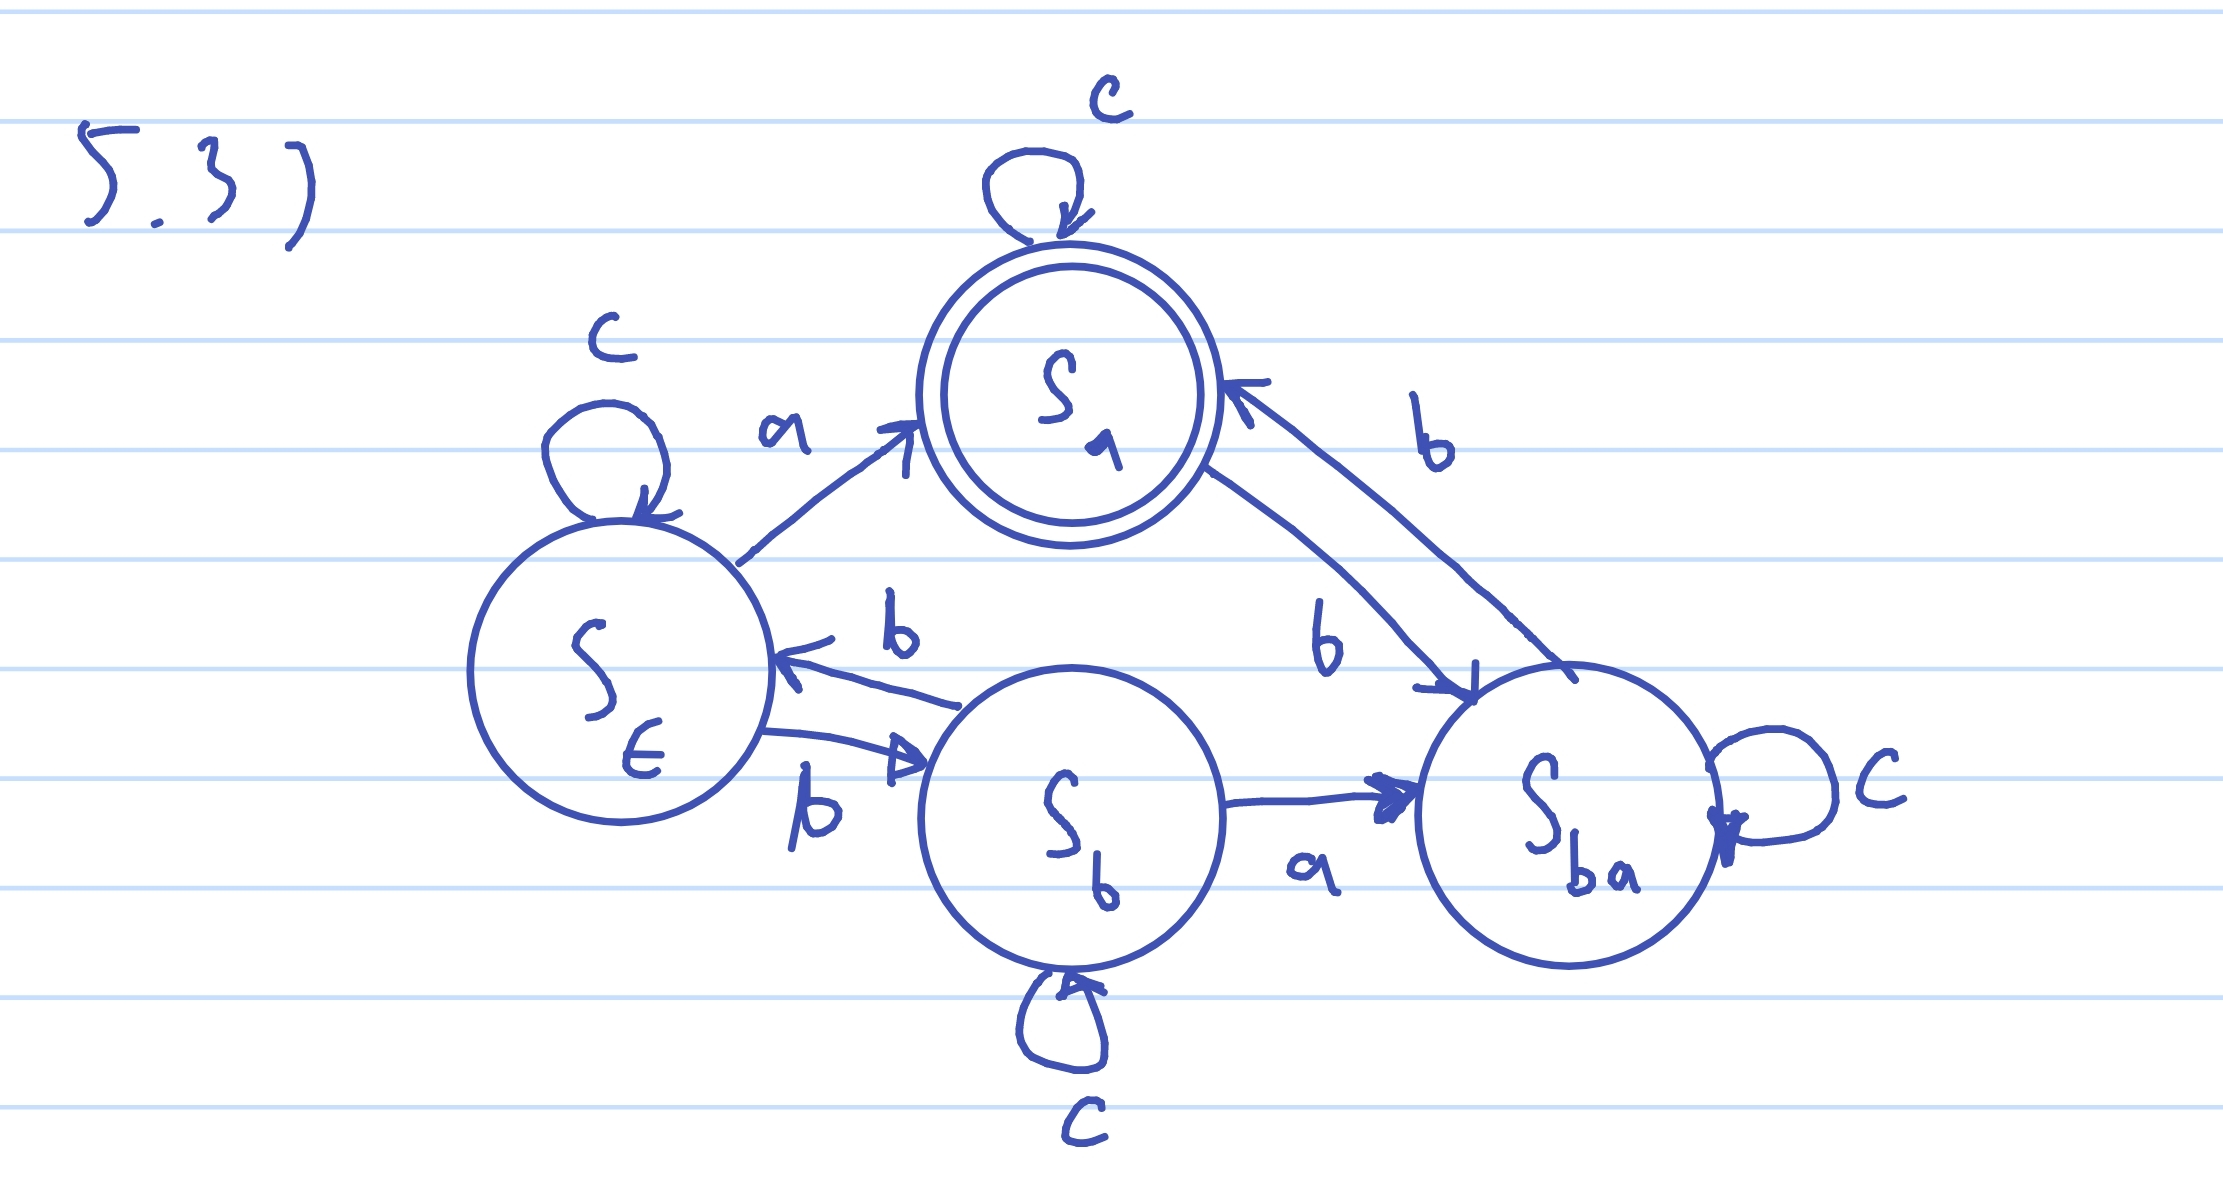
\includegraphics[width=\linewidth]{figures/3.jpg}
	\end{figure}

	Let $K$ be any input string from language set $\sum$.
	
	$S_\epsilon$ represents the state where there is not a match with the pattern.\\
	$S_a$ represents the state where K has at least one $a$ and contains an even number of $b$s.\\
	$S_{ba}$ represents the state where K has at least one $a$ and contains an odd number of $b$s.\\
	$S_b$ represents the state where K has no $a$ and contains an odd number of $b$s.
	
	So, the accepting state is $S_a$ since this state means the input string has at least one $a$ and contains an even number of $b$s.
	\\\\\\\\\\\\\\\\\\\\\\\\\\
	
	
	\question{6}{Penultimate}
	\part{1} Let $L_2 = \{x \in \sum^{*}: \text{the 2nd-to-last symbol of x is 1}\}$. Draw a DFA with 4 states that accepts $L_2$.
	
	{\em Solution}:
	\begin{figure}[htbp]
		\centering
		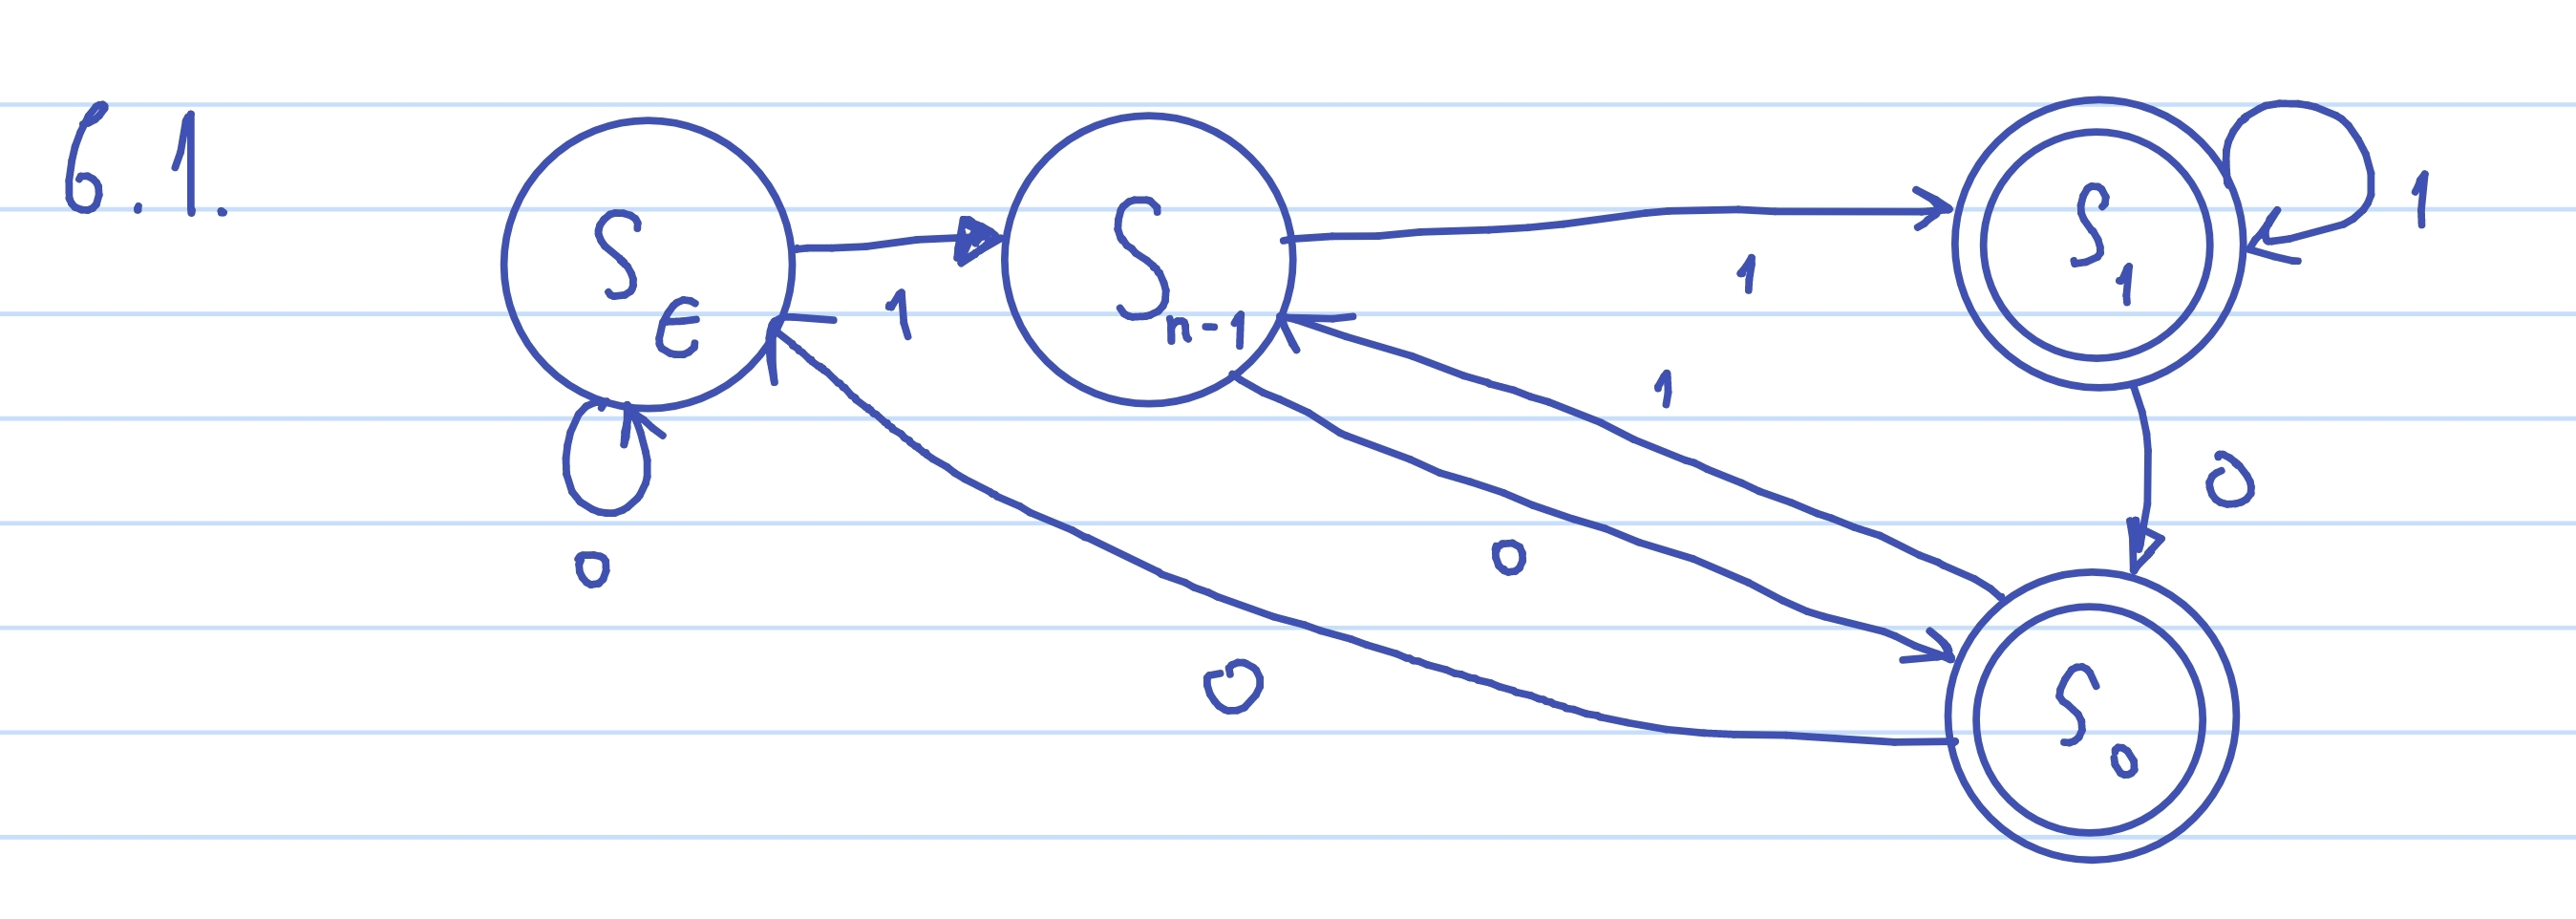
\includegraphics[width=\linewidth]{figures/4.jpg}
	\end{figure}
	
	$S_\epsilon$ represents the state where there is not a match with the pattern.\\
	$S_{n-1}$ represents the state where $1$ is found but at the last position.\\
	$S_{1}$ represents the state where $1$ is found at the second-to-last position, and the last alphabet is $1$.\\
	$S_0$ represents the state where $1$ is found at the second-to-last position, and the last alphabet is $0$.\\
	
	So, the accepting state is $S_1 \text{ and } S_0$ since these states mean the second-to-last symbol of input string is $1$.
	
	
	\part{2} Show that any DFA that correctly recognizes $L_2$ must have at least 4 states.
	
	{\em Proof}: Without loss of generality, let us assume for the sake of contradiction that there exist D, a DFA that correctly recognizes $L_2$ using less than 4 states. Let D be a DFA that has 3 states. So, to check whether a string can be recognize requires 4 steps. 
	The first step is to check whether we found 1 yet, because it could the the second last position symbol we need. 
	The second step is to check whether the next state is 1 or zero, and there will be two cases to consider, the first case is that the second-to-last symbol of $x$ is 1 and the next symbol is 1 and another case is the second-to-last symbol of $x$ is 1 and the next symbol is 0. We have to change state every time any 0 showed up after we found the first 1. So, we need at least 4 steps to correctly recognize $L_2$. Using pigeonhole principle, the least number of states required is 4 since we showed that 4 different states are needed but the number of states in D is smaller than 4 and there are some patterns of symbols such as 1010 and 1101 that could end up in the same state. Hence, D cannot correctly recognize $L_2$ with only 3 states which is contradicting to what our assumption.
	
	Therefore, any DFA that correctly recognizes $L_2$ must have at least 4 states. $\square$
	\\\\\\\\\\
	\question{7}{Digit Sum}
	\part{1} $L = \{x \in \sum^{*}: \texttt{DIGITSUM(x)} \text{is divisible by 3}\}$. Draw a DFA that recognizes $L$. Explain what each of your states represents.
	
	{\em Solution}:
	\begin{figure}[htbp]
		\centering
		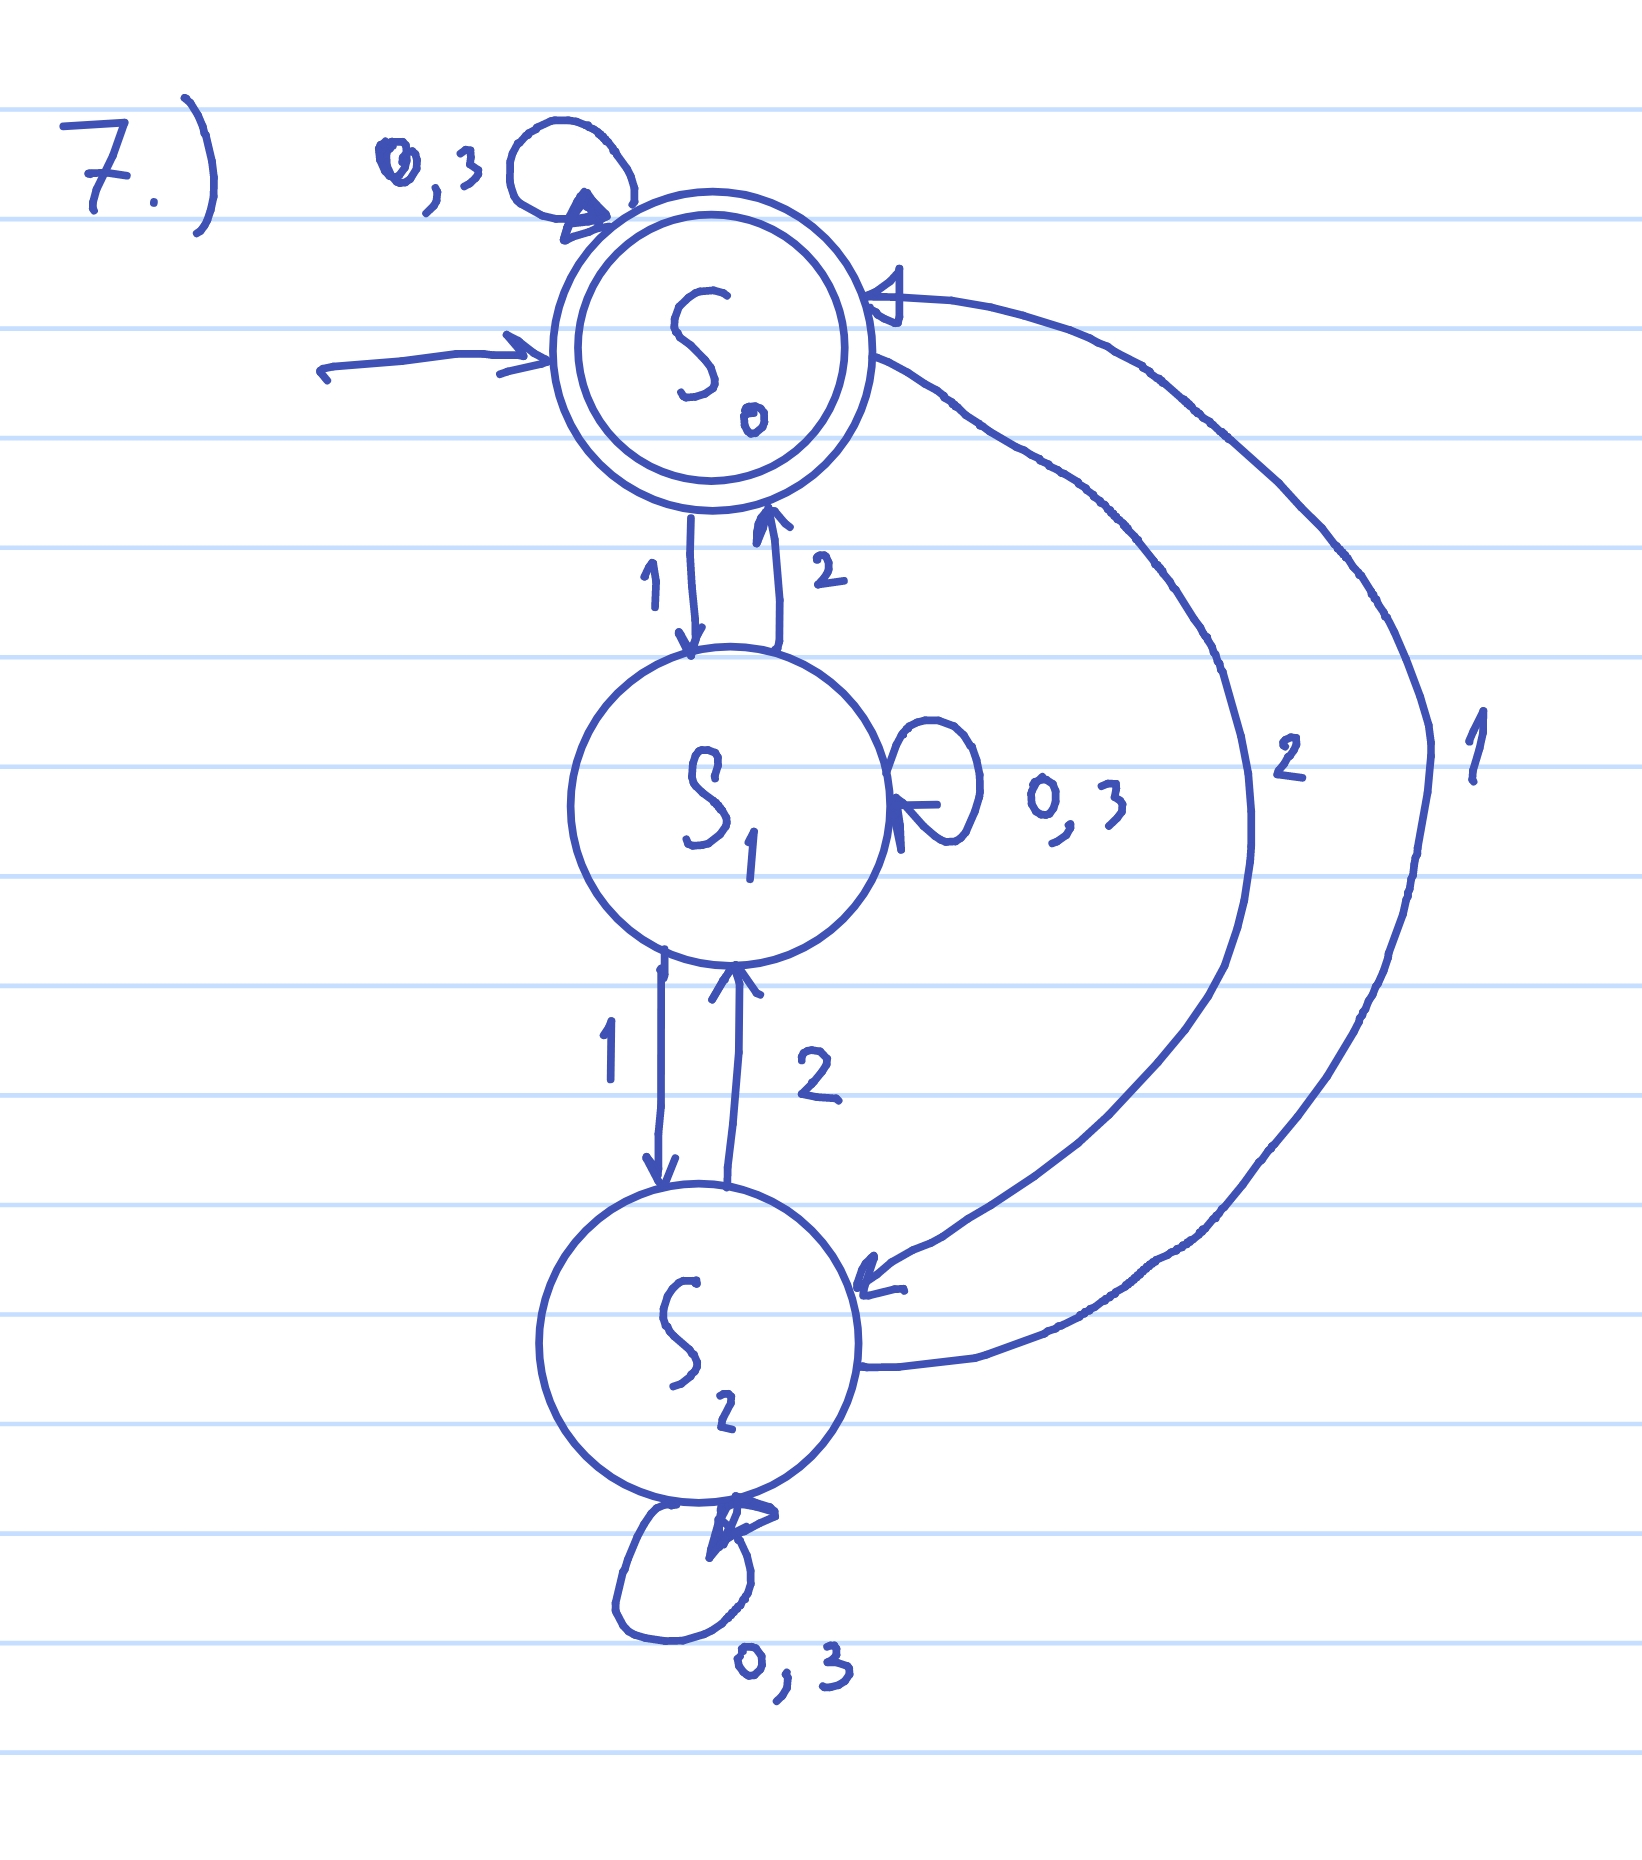
\includegraphics[width=400px]{figures/5.jpg}
	\end{figure}
	
	Let $n_i$ be the accumulating sum of input string at position $i$.
	
	$S_0$ represents the state where $0 \pmod{3} \equiv n_i$.\\
	$S_1$ represents the state where $1 \pmod{3} \equiv n_i$.\\
	$S_2$ represents the state where $2 \pmod{3} \equiv n_i$.\\
	
	So, the accepting state is $S_0$ since this state means $\texttt{DIGITSUM(x)} \text{is divisible by 3}$ where $x \in \sum^{*}$.
\end{document}